%%%%%%%%%%%%%%%%%%%%%%%%%%%%%%%%%%%%%%%%%%%%%%%%%%%%%%
\documentclass[11pt]{article}
%%%%%%%%%%%%%%%%%%%%%%%%%%%%%%%%%%%%%%%%%%%%%%%%%%%%%%

\usepackage{amsmath}
\usepackage{amsthm}
\usepackage{amssymb}
\usepackage{latexsym}
\usepackage{graphicx}
\usepackage{color}
\usepackage{verbatim}
\usepackage{float}
\usepackage{multicol}
\usepackage{xcolor}
\usepackage{listings}
\usepackage{tikz}
\usetikzlibrary{arrows.meta, positioning, calc}
\usetikzlibrary{decorations.pathmorphing}
\usepackage{tcolorbox}
\tcbuselibrary{breakable}

\newtcolorbox{solutionbox}{
  breakable,
  colback=blue!5!white,
  colframe=blue!50!black,
  title=Solution,
  sharp corners,
  boxrule=0.8pt
}

\newtcolorbox{hintbox}{
  breakable,
  colback=gray!10!white,
  colframe=gray!50!black,
  title=Hint,
  sharp corners,
  boxrule=0.5pt
}

% Unnumbered theorem
\newtheorem*{thm*}{Theorem}


\lstdefinelanguage{R}{
      keywords={if,else,while,for,in,next,break,function,TRUE,FALSE,NULL,Inf,NA,NaN,switch,repeat,return,require,library},
      keywordstyle=\color{blue}\bfseries,
      identifierstyle=\color{black},
      comment=[l]{\#},
      commentstyle=\color{gray}\ttfamily,
      string=[b]{"},
      stringstyle=\color{red}\ttfamily,
      morecomment=[l]{//},
      morestring=[b]{'},
      sensitive=true,
      morekeywords={print,summary,plot,lm,glm,data,frame,read.csv,write.csv,factor,levels,names,colnames,rownames,
      head,tail,str,dim,length,class,typeof,mode,is.na,is.null,is.finite,is.infinite,is.nan,as.numeric,as.character,
      as.factor,as.Date,as.POSIXct,as.matrix,as.data.frame,rbind,cbind,merge,subset,aggregate,tapply,apply,lapply,sapply,
      mapply,vapply,replicate,seq,rep,c,list,matrix,array,data.frame,table,hist,boxplot,barplot,pie,curve,lines,points,text,
      abline,legend,par,mtext,title,xlab,ylab,xlim,ylim,main,sub,col,pch,cex,lty,lwd,type,bg,fg,args,options,warnings,errors,
      message,stop,warning,error,try,tryCatch,withCallingHandlers,on.exit,debug,browser,trace,recover,options,getOption,setOption},
    }


\setlength{\textheight}{9in}
\setlength{\textwidth}{6in}
\addtolength{\topmargin}{-2cm}
\addtolength{\oddsidemargin}{-1cm}
\parindent=0in


\def\classnum{3810}
\def\classtitle{Probability}
\def\classtitleshort{Probability}
\def\classsec{001}
\def\classterm{Fall 2025}
\def\instructor{Robert Rostermundt}
%\def\hmwknum{\#2}


%%%%%%%%%%%%%%%%%%%%%%%%%%%%%%%%%%%%%%%%%%%%%%%%%%%%%%%%%
%%%%%%%%%%%%%%%%%%%%%%%%%  Colors  %%%%%%%%%%%%%%%%%%%%%%
%%%%%%%%%%%%%%%%%%%%%%%%%%%%%%%%%%%%%%%%%%%%%%%%%%%%%%%%%

\definecolor{Green}{rgb}{0,.5,0}
%use for definitions
\definecolor{Red}{rgb}{.8,.2,0}
%use for emphasis
\definecolor{Yellow}{rgb}{.6,.6,.1}
%use for part titles
\definecolor{Cyan}{rgb}{.2,.6,.7}
%use for comments
\definecolor{Purple}{rgb}{.4,0,1}
%use for examples
\definecolor{deepred}{rgb}{.53,.29,.24}
%use for important points
\definecolor{Black}{rgb}{0,0,0}
%use for washout
\definecolor{Grey}{rgb}{.45,.45,.45}
% use for theorems
\newcommand{\tred}[1]{\textcolor{Red}{#1}}
\newcommand{\tgreen}[1]{\textcolor{Green}{#1}}
\newcommand{\tcyan}[1]{\textcolor{Cyan}{#1}}
\newcommand{\tyellow}[1]{\textcolor{Yellow}{#1}}
\newcommand{\tpurple}[1]{\textcolor{Purple}{#1}}
\newcommand{\tblack}[1]{\textcolor{Black}{#1}}
\newcommand{\tgrey}[1]{\textcolor{Grey}{#1}}
\newcommand{\tdeepred}[1]{\textcolor{deepred}{#1}}
\newcommand{\ttt}[1]{\texttt{#1}}

%%%%%%%%%%%%%%%%%%%%%%%%%%%%%%%%%%%%%%%%%%%%%%%%%%%%%%%%%
%%%%%%%%%%%%%%%%%%%%%%%%%  Theorem Environments  %%%%%%%%
%%%%%%%%%%%%%%%%%%%%%%%%%%%%%%%%%%%%%%%%%%%%%%%%%%%%%%%%%

\theoremstyle{plain}
\newtheorem{thm}{Theorem}
\newtheorem{axiom}{Axiom}
\newtheorem{cor}{Corollary}
\newtheorem{lemma}{Lemma}
\newtheorem{prop}{Proposition}
\newtheorem{ques}{Question}
\theoremstyle{definition}
\newtheorem{defn}{Definition}
\theoremstyle{remark}
\newtheorem{remark}{Remark}
\theoremstyle{definition}
\newtheorem{ex}{Example}
\numberwithin{equation}{section}
\newtheorem{prob}{Problem}
\numberwithin{equation}{section}


%%%%%%%%%%%%%%%%%%%%%%%%%%%%%%%%%%%%%%%%%%%%%%%%%%%%%%%%%
%%%%%%%%%%%%%%%%%%%%%%%%%  Math    %%%%%%%%%%%%%%%%%%%%%%
%%%%%%%%%%%%%%%%%%%%%%%%%%%%%%%%%%%%%%%%%%%%%%%%%%%%%%%%%


\newcommand{\abs}[1]{\left\lvert{#1}\right\rvert}
\newcommand{\card}[1]{\lvert{#1}\rvert}
\newcommand{\union}{\cup}
\newcommand{\Union}{\bigcup}
\newcommand{\inter}{\cap}
\newcommand{\Inter}{\bigcap}
%\newcommand{\hint}[1]{\medskip\newline\emph{Hint: #1}}
%\newcommand{\note}[1]{\medskip\newline\emph{Note: #1}}
\newcommand{\points}[1]{[#1 points]}
\newcommand{\totalpoints}[1]{[#1 points total]}
\newcommand{\ds}{\displaystyle}
\newcommand{\ben}{\begin{enumerate}}
\newcommand{\een}{\end{enumerate}}
\newcommand{\bi}{\begin{itemize}}
\newcommand{\ei}{\end{itemize}}
\newcommand{\beq}{\begin{eqnarray*}}
\newcommand{\eeq}{\end{eqnarray*}}
\newcommand{\bieq}{\begin{IEEEeqnarray}{rCl}}
\newcommand{\bieqx}{\begin{IEEEeqnarray}{+rCl+x*}}
\newcommand{\eieq}{\end{IEEEeqnarray}}
\newcommand{\nn}{\nonumber}
%\renewcommand{\i}{\item}
\newcommand{\bpm}{\begin{pmatrix}}
\newcommand{\epm}{\end{pmatrix}}
\newcommand{\sol}{\indent{\bf\emph{Solution:}}}
\newcommand{\ssol}{\indent{\\[2mm]\bf\emph{Solution:}}\;}
\newcommand{\hint}{\indent{\bf\emph{Hint}:}\;}
\newcommand{\note}{\indent{\bf\emph{Note}:}\;}
\newcommand{\vsk}{\vskip 2mm}
%%%%%%%%%%%%%%%%%%%%%%%%% Calculus %%%%%%%%%%%%%%%%%%%%%%%%%%%%
\newcommand{\dd}[2]{\ds\frac{d}{d{#1}}\left[{#2}\right]}
\newcommand{\der}[2]{\ds\frac{d{#1}}{d{#2}}}
\newcommand{\lmt}[3]{\ds\lim_{{#1}\to{#2}}{#3}}
\renewcommand{\iint}[2]{\ds\int{#1}\,d{#2}}
\newcommand{\dint}[4]{\ds\int^{#4}_{#3}{#1}\,d{#2}}
\renewcommand{\Delta}{\triangle}
%%%%%%%%%%%%%%%%%%%%%%%%% Number Sets %%%%%%%%%%%%%%%%%%%%%%%%%%
\newcommand{\N}{\mathbb{N}}
\newcommand{\Z}{\mathbb{Z}}
\newcommand{\Q}{\mathbb{Q}}
\newcommand{\R}{\mathbb{R}}
\newcommand{\C}{\mathbb{C}}
\newcommand{\F}{\mathcal{F}}
\renewcommand{\P}{\mathbb{P}}
\newcommand{\E}{\mathcal{E}}
\renewcommand{\o}{\omega}
\renewcommand{\O}{\Omega}
%%%%%%%%%%%%%%%%%%%%%%%%% Vectors %%%%%%%%%%%%%%%%%%%%%%%%%%%%%
\newcommand{\x}{\bar{x}}
\renewcommand{\v}{\bar{v}}
\newcommand{\y}{\bar{y}}
\newcommand{\z}{\bar{z}}
\newcommand{\w}{\bar{w}}
\renewcommand{\u}{\bar{u}}
\renewcommand{\b}{\bar{b}}
\newcommand{\e}{\bar{e}}
\renewcommand{\a}{\vec{a}}
\renewcommand{\r}{\vec{r}}
\newcommand{\vv}{\vec{v}}
\newcommand{\vecPQ}[2]{\overrightarrow{#1}{#2}}
\newcommand{\vecV}[1]{\overrightarrow{#1}}
\newcommand{\la}{\langle}
\newcommand{\ra}{\rangle}
%%%%%%%%%%%%%%%%%%%%%%%%%%% Vector Spaces %%%%%%%%%%%%%%%%%%%%
\newcommand{\rn}{\ensuremath{\mathbb{R}^n}}
\renewcommand{\rm}{\ensuremath{\mathbb{R}^m}}
\newcommand{\re}{\mathbb{R}}
\newcommand{\Pn}{\mathbb{P}_n}
\newcommand{\B}{\mathcal{B}}
%%%%%%%%%%%%%%%%%%%%%%%%%%% Graphics %%%%%%%%%%%%%%%%%%%%%%%%
\newcommand{\cg}[2]{\begin{center}
\includegraphics[scale={#1}]{{#2}}
\end{center}}
\makeatletter
\def\imod#1{\allowbreak\mkern10mu({\operator@font mod}\,\,#1)}
\makeatother

%%%%%%%%%%%%%%%%%%%%%%%%%%%%%%%%%%%%%%%%%%%%%%%%%%%%%%%%%%%%%%%%%%%%%%%%%%%%%%%%%%%%%%%%%%%%%%
%%%%%%%%%%%%%%%%%%%%%%%%%%%%%% Defined Fonts %%%%%%%%%%%%%%%%%%%%%%%%%%%%%%%%%%%%%%%%%%%%%%%%%
%%%%%%%%%%%%%%%%%%%%%%%%%%%%%%%%%%%%%%%%%%%%%%%%%%%%%%%%%%%%%%%%%%%%%%%%%%%%%%%%%%%%%%%%%%%%%%

\font\minihelv=phvr at 6pt
\font\helv=phvr at 10pt
\font\medhelv=phvr at 16pt
\font\bighelv=phvr at 20pt
\font\hugehelv=phvr at 36pt
\font\mybigfont=phvr at 16pt
\font\mymediumfont=phvr at 14pt
\font\mediumhelv=phvr at 14pt
\font\mybfit=ptmbi at 12pt


%%%%%%%%%%%%%%%%%%%%%%%%%%%%%%%%%%%%%%%%%%%%%%%%%%%%%%%%%%%%%%%%%%%%%%%%%%%%%%%%%%%%%%%%%%%%%%%
%%%%%%%%%%%%%%%%%%%%%%%%%%%%%% Other Commands %%%%%%%%%%%%%%%%%%%%%%%%%%%%%%%%%%%%%%%%%%%%%%%%%
%%%%%%%%%%%%%%%%%%%%%%%%%%%%%%%%%%%%%%%%%%%%%%%%%%%%%%%%%%%%%%%%%%%%%%%%%%%%%%%%%%%%%%%%%%%%%%%
%\setlength\fboxrule{.5pt}
%\newcommand{\latexpicborder}[3]{
%\setlength\fboxsep{30pt}
%\begin{figure}[hb]
%\begin{center}
%\fbox{
%\input{#1}
%}
%\caption{#2}
%\label{#3}
%\end{center}
%\end{figure}
%\setlength\fboxsep{0pt}
%}
%
%\newcommand{\latexpic}[2]{
%\begin{figure}[hb]
%\begin{center}
%\input{#1}
%\vspace*{8mm}
%\caption{#2}
%\end{center}
%\end{figure}
%}

%\begin{minipage}[b]{0.6\linewidth}
%......
%\end{minipage}
%\hspace{0.5cm}
%\begin{minipage}[t]{0.4\linewidth}
%\centering
%\includegraphics[scale=.5]{m1401_ex3_g4.eps}
%\end{minipage}
%\end{figure}


%%%%%%%%%%%%%%%%%%%%%%%%%%%%%%%%%%%%%%%%%%%%%%%%%%%%%%%%%%%%%%%%%%%%%%%%%%%%%%%%%%%%%%%%%%%%%%
%%%%%%%%%%%%%%%%%%%%%%%%%%% IEEEeqnarray Notes %%%%%%%%%%%%%%%%%%%%%%%%%%%%%%%%%%%%%%%%%%%%%%%
%%%%%%%%%%%%%%%%%%%%%%%%%%%%%%%%%%%%%%%%%%%%%%%%%%%%%%%%%%%%%%%%%%%%%%%%%%%%%%%%%%%%%%%%%%%%%%


%Any number of columns can be specified with IEEEeqnarray: {c} will give only one
%column with all entries centered, or {rCll} would add a fourth, left-justified
%column to use for comments. Moreover, beside l, c, r, L, C, R for math mode
%entries there are also s, t, u for left, centered, and right text mode entries.
%Additional space can be added with . and / and ? in increasing order.
%
%
%\begin{proof}
%This is a proof that ends
%with an equation array:
%\begin{IEEEeqnarray*}{+rCl+x*}
%a & = & b + c \\
%& = & d + e. & \qedhere
%\end{IEEEeqnarray*}
%\end{proof}
%Note that the + in {+rCl+x*} denotes stretchable spaces, one on the left
%of the equations (which, if not specified, will be done automatically by
%IEEEeqnarray!) and one on the right of the equations. But now on the right,
%after the stretching column, we add an empty column x. This column will be
%only needed on the last line when we will put the \qedhere command there.
%Finally, we specify a *. This is a null-space that prevents IEEEeqnarray to
%add another unwanted +-space!


% The following environments enable custom numbering of theorems so that the numbers agree % with the numbering in the textbook being used. 
%
%  Usage examples:
%\begin{customthm}{2.2}\label{eight}
%Every theorem must be numbered by hand.
%\end{customthm}
%
%Here is a reference to theorem~\ref{eight}.
%
%\begin{customthm}{2.3}[Parenthetical comment]\label{nine}
%Statement
%\end{customthm}
%
%Here is a reference to theorem~\ref{nine}


\newtheorem{innercustomthm}{Theorem}
\newenvironment{customthm}[1]
  {\renewcommand\theinnercustomthm{#1}\innercustomthm}
  {\endinnercustomthm}
  
  \newtheorem{innercustomprop}{Proposition}
\newenvironment{customprop}[1]
  {\renewcommand\theinnercustomprop{#1}\innercustomprop}
  {\endinnercustomprop}
  
    \newtheorem{innercustomlem}{Lemma}
\newenvironment{customlem}[1]
  {\renewcommand\theinnercustomlem{#1}\innercustomlem}
  {\endinnercustomlem}
  
    \newtheorem{innercustomconj}{Conjecture}
\newenvironment{customconj}[1]
  {\renewcommand\theinnercustomconj{#1}\innercustomconj}
  {\endinnercustomconj}
  
    \newtheorem{innercustomclaim}{Claim}
\newenvironment{customclaim}[1]
  {\renewcommand\theinnercustomclaim{#1}\innercustomclaim}
  {\endinnercustomclaim}
  
    \newtheorem{innercustomcor}{Corollary}
\newenvironment{customcor}[1]
  {\renewcommand\theinnercustomcor{#1}\innercustomcor}
  {\endinnercustomcor}
  
    \newtheorem{innercustomdef}{Definition}
\newenvironment{customdef}[1]
  {\renewcommand\theinnercustomdef{#1}\innercustomdef}
  {\endinnercustomdef}
  
    \newtheorem{innercustomex}{Example}
\newenvironment{customex}[1]
  {\renewcommand\theinnercustomex{#1}\innercustomex}
  {\endinnercustomex}
  
    \newtheorem{innercustomass}{Assumption}
\newenvironment{customass}[1]
  {\renewcommand\theinnercustomass{#1}\innercustomass}
  {\endinnercustomass}
  
      \newtheorem{innercustomax}{Axiom}
\newenvironment{customax}[1]
  {\renewcommand\theinnercustomax{#1}\innercustomax}
  {\endinnercustomax}
  

\vfuzz2pt % Don't report over-full v-boxes if over-edge is small
\hfuzz2pt % Don't report over-full h-boxes if over-edge is small

\renewcommand{\ni}{\noindent}


%%%%%%%%%%%%%%%%%%%%%%%%%%%%%%%%%%%%%%%%%%%%%%%%%%%%%%
%%%%%%%%%%%%%%%%%%%%%%%%%%%%%%%%%%%%%%%%%%%%%%%%%%%%%%

\pagestyle{myheadings}

%%%%%%%%%%%%%%%%%%%%%%%%%%%%%%%%%%%%%%%%%%%%%%%%%%%%%%

%%%%%%%%%%%%%%%%%%%%%%%%%%%%%%%%%%%%%%%%%%%%%%%%%%%%%%
%%%%%%%%%%%%%%%%%%%%%%%%%   Document Body   %%%%%%%%%%
%%%%%%%%%%%%%%%%%%%%%%%%%%%%%%%%%%%%%%%%%%%%%%%%%%%%%%

%\def\classnum{3810}
%\def\classtitle{Probability}
%\def\classtitleshort{Probability}
%\def\classsec{001}
%\def\classterm{Fall 2025}
%\def\instructor{Robert Rostermundt}
\def\printsol{0}
\def\printsol{0}


	\title{\vspace{-1in}Math\classnum\;-\;\classtitle\\
	Section\;\classsec\;-\;\classterm\\
	Notes: Probability Axioms and Properties}
	\author{University of Colorado Denver / College of Liberal Arts 	and Sciences}
	\date{Department of Mathematics - \instructor}

	\markright{Math\classnum\;-\;\classtitleshort, UCD, \classterm, \instructor}



%%%%%%%%%%%%%%%%%%%%%%%%%%%%%%%%%%%%%%%%%%%%%%%%%%%%%%
\begin{document}\maketitle\thispagestyle{empty}
%%%%%%%%%%%%%%%%%%%%%%%%%%%%%%%%%%%%%%%%%%%%%%%%%%%%%%



%%%%%%%%%%%%%%%%%%%%%%%%%%%%%%%%%%%%%%%%%%%%%%%%%%%%%%%%%%%%%%%%%%%%%%%%%%%%%%%%%%%%%%%%%%%%%%%%%%%%%%
\vspace*{2mm}
\hrule
\vskip 8mm


%%%%%%%%%%%%%%%%%%%%%%%%%%%%%%%%%%%%%%%%%%%%%%%%%%%%%%%%%%%%%%%%%%%%%%%%%
%%%%%%%%%%%%%%%%%%%%%%%%%%%%%%%%%%%%%%%%%%%%%%%%%%%%%%%%%%%%%%%%%%%%%%%%%


%%%%%%%%%%%%%%%%%%%%%%%%%%%%%%%%%%%%%%%%%%%%%%%%%%%%%%%%%%%%%%%%%%%%%%%%%%%%%%%%%%%%%%%%%%%%%%%%%%%%%%
\section*{Probability Foundations:}
%%%%%%%%%%%%%%%%%%%%%%%%%%%%%%%%%%%%%%%%%%%%%%%%%%%%%%%%%%%%%%%%%%%%%%%%%%%%%%%%%%%%%%%%%%%%%%%%%%%%%%


\noindent Probability is a measure of our beliefs about the likelihood of certain events such as the likelihood that we obtain heads on single flip of a coin. Of particular interest in applications, we might want an experimental method to determine an unknown probability or likelihood. For example, consider the following simple experiment. Suppose we are given a coin and asked to determine the probability of obtaining heads on a single flip of the coin. Our experimental procedure to determine this probability might consist of multiple coin flips and dividing the number of heads by the total number of coin flips. This ratio would then be considered as an estimate of the true probability of obtaining heads. Intuitively, we believe that there is a well-defined probability for such an outcome, and we believe that the greater the number of coin flips in the above experiment the closer we should be to the actual probability (or likelihood) of obtaining heads on a single flip of the coin. We might write this formally in the following manner. Let $H_n$ be the number of heads in $n$ flips of the coin. Then
\[\P(\text{Heads on a single coin flip})=\ds\lim_{n\to\infty}\ds\frac{H_n}{n}.\]
This is what is known as a ``frequency interpretation" of probability. But how do we know that the above limit actually exists? Are we certain that the ratio converges to some value? If we run the process multiple times will we always converge to the same value?\\

\ni In these notes we aim to verify the correctness of this experimental method using a rigorous mathematical approach to probability. (Moreover, we will see some of the consequences and applications of this frequency approach, such as simulations and Monte Carlo procedures.) To do this we will use an axiomatic mathematical framework which is built on abstract notions of probability spaces and random variables. In this section we review the foundations for such a mathematical probability theory, assuming that the reader has some familiarity with basic probability theory, as well as a basic familiarity with properties of real numbers such as cardinality (the rational numbers form a countable set and can therefore be listed in a sequence, where the real numbers are uncountable and so can not be listed in a sequence).\\

\ni We start with an experiment $\E$ (such as flipping a coin, rolling dice, etc.). Then given the experiment $\E$ we first define the {\bf\emph{sample space}} $\O$ to be the set of all possible {\bf\emph{outcomes}} of the experiment $\E$. That is,
\[\O=\{\text{all possible outcomes of the experiment}\;\E\}.\]
We then define the {\bf\emph{event space}} $\F$ to be a collection of subsets of the sample space $\O$ that are of interest to us. We call the elements of $\F$ the {\bf\emph{events}}. We will soon revisit the event space $\F$ and consider restrictions that should be applied to this collection. It turns out that the proper way to assign probabilities is not to the individual outcomes (especially when considering uncountable sample spaces since in this case the probability of a single outcome must be equal to zero), but rather to the events of $\F$. Therefore, we will define a {\bf\emph{probability measure}} $\P$ to be a function from the event space to the interval $[0,1]$ that satisfies certain axioms. That is, a probability measure is a set-function $\P:\F\to[0,1]$ such that the following axioms are satisfied:
\begin{enumerate}
\item $\P(\emptyset)=0$;
\item $\P(\O)=1$;
\item If $A_1,A_2,A_3,\dots$ is a countably infinite sequence of mutually disjoint events in $\F$; i.e., $A_k\bigcap A_j=\emptyset$ when $k\not=j$, then $\P\left(\ds\bigcup^{\infty}_{i=1}A_i\right)=\ds\sum^{\infty}_{i=1}\P(A_i)$.
\end{enumerate}

\ni We want property(iii) for situations such as where $\O=(0,1]$ and $A_i=(1/(i+1),1/i]$ for $i=1,2,3,\dots$. Then $\cup_{i}A_i=\O$ and we would like to have $\P\big(\cup_{i}A_i\big)=\sum_{i}|1/i-1/(i+1)|=|(0,1]|=1$.\\ 

\ni Now that we have defined the sample space $\O$, the event space $\F$, and a probability measure $\P$, we now can define a {\bf\emph{probability space}} to be the triple $(\O,\F,\P)$.\\

\ni We are now ready to consider desired properties of our event space $\F$ (which is the domain of the function $\P$). Because we are assigning probabilities to events in a way that satisfies the probability axioms, at a minimum we would like the following to hold: (1) $\emptyset\in\F$; (2) $\Omega\in\F$; (3) if $A\in\F$, then $A^C\in\F$; (4) and if $A_1,A_2,A_3,\dots$ is a countably infinite sequence of events in $\F$, then $\cup^{\infty}_{i=1}A_i\in\F$.\\ 

\ni {\bf\emph{Note}:} We want property(3) because if $A\in\F$ and we can assign $\P(A)$, we also want to be able to assign a probability $P(A^C)$ (where $A^C$ is the event that $A$ does not occur). 

\begin{defn}
We define a $\sigma$-algebra to be a non-empty collection $\F$ of subsets of $2^{\O}$ (the power set of a set $\O$) so that the following hold.
\begin{enumerate}
\item $\O\in\F$;
\item If $A\in\F$, then $A^C\in\F$.
\item If $A_1,A_2,A_3,\dots$ is a countably infinite sequence of events in $\F$, then $\bigcup^{\infty}_{i=1}A_i\in\F$.
\end{enumerate}
\end{defn}

\ni So $\F$ is closed under compliments and under countable unions. We have the following consequences in the next theorem which we offer without proof.\\

\begin{thm}
Let $\F$ be a $\sigma$-algebra the is a collection of subsets of $\O$. Then the following hold.

	\begin{enumerate}
		\item $\emptyset\in\F$.
		\item If $A_1,A_2,A_3,\dots,A_n$ is a finite sequence of events in $\F$, then $\bigcup^{n}_{i=1}A_i\in\F$. So $\F$ is closed under finite unions.	
		\item If $A_1,A_2,A_3,\dots,A_n$ is a finite sequence of events in $\F$, then $\bigcap^{n}_{i=1}A_i\in\F$. So $\F$ is closed under finite intersections.
		\item If $A_1,A_2,A_3,\dots$ is a countably infinite sequence of events in $\F$, then $\bigcap^{\infty}_{i=1}A_i\in\F$.
	\end{enumerate}

\end{thm}

\ni The point is that we will want our event space $\F$ to be a $\sigma$-algebra. The simplest examples of $\sigma$-algebras would be $\F=\{\emptyset,\O\}$ or $\F=2^{\O}$. The first example is trivial and of little use. The second example contains all information from the power set of $\O$, but is often too large a $\sigma$-algebra to satisfy the probability axioms. Actually, if $\O$ is a discrete sample space (so that there are either a finite number of elements in $\O$ or a countably infinite number of elements in $\O$) will will generally choose $\F$ to be the power set of $\O$. However, if $\O$ is a continuous sample space, then we can never choose $\F$ to be the power set of $\O$. We will soon provide the reader with an explanation, but first we need some background, which we motivate with an example.\\

\ni Suppose that we have the probability space $(\O,\F,\P)$, where $\O=(0,1]$ is the half-closed interval on the real line, and $\P$ is a uniform probability measure. (For a uniform probability measure we want the probability for an interval to be proportional to the length of that interval.) Then, if $(a,b]$ is a sub-interval of $(0,1]$, we will define $\P[(a,b]]=b-a$. So, in general, for any element $A\in\F$ we would like $\P(A)$ to be equal to the ``length" of $A$, denoted $|A|$. We would also like $\P$ to be invariant under translation. That is, $\P(A)=\P(A\oplus c)$, for any constant $c$ where we define the sum $A\oplus c$ to be
\[A\oplus c=\big\{a+c:a\in A,\;\;a+c\le 1\big\}\cup
\big\{a+c-1:a\in A,\;\;a+c\ge 1\big\}.\]
But then what about the a set such as $A=\Q\cap(0,1]$, the set of all rational numbers in the interval $[0,1]$? How do we compute $\P(A)$ given that we want $\P(A)=|A|$? We clearly need to generalize our notion of ``length", but in a manner that is consistent with our current measure of length of intervals. We will call this generalization a {\bf\emph{measure}}, which will be a function
\[\mu^*:2^{\R}\to[0,\infty].\]

%%%%%%%%%%%%%%%%%%%%%%%%%%%%%%%%%%%%%%%%%%%%%%%%%%%%%%%%%%%%%%%%%%%%%%%%%%%%%%%%%%%%%%%%%%%%%%%%%%%%%%
\section*{Consequences of the Probability Axioms:}
%%%%%%%%%%%%%%%%%%%%%%%%%%%%%%%%%%%%%%%%%%%%%%%%%%%%%%%%%%%%%%%%%%%%%%%%%%%%%%%%%%%%%%%%%%%%%%%%%%%%%%

\noindent Given our probability axioms, for any probability space $(\O,\F,\P)$ we have the following properties, most of which are listed without proof.

	\begin{enumerate}
	
		\item {\bf\emph{Finite Additivity}}: If $A_1,A_2,\dots,A_n$ is a list of disjoint events, then $\P\left(\ds\bigcup^{n}_{i=1}A_i\right)=\ds\sum^{n}_{i=1}\P(A_i)$.

		\item {\bf\emph{Compliments}}: For any event $A\in\F$, we have $\P(A^C)=1-\P(A)$.
		
		\item {\bf\emph{Monotonicity}}: If $A,B\in\F$ and $A\subseteq B$, then $\P(A)\le\P(B)$.
		
		\item {\bf\emph{Unions}}: If $A,B\in\F$, then $\P\left(A\ds\cup B\right)=\P(A)+\P(B)-\P(A\ds\cap B)$.
		
		\item {\bf\emph{Inclusion-Exclusion}}: If $A_1,A_2,\dots,A_n\in\F$, then we have
		\[\P\left(\ds\bigcup^{n}_{i=1}A_i\right)=\ds\sum^{n}_{i=1}\P(A_i)- \ds\sum_{i\not=j}\P\left(A_i\ds\cap A_j\right)+\ds\sum_{i\le j\le k}\P\left(A_i\ds\cap A_j\ds\cap A_k\right)+\cdots+ (-1)^{n-1}\P\left(\ds\bigcap^{n}_{i=1}A_i\right).\]
		
		\item {\bf\emph{Continuity}}: If $A_1,A_2,\dots\in\F$, then $\P\left(\ds\bigcup^{\infty}_{i=1}A_i\right)=\ds\lim_{n\to\infty}\P\left(\ds\bigcup^{n}_{i=1}A_i\right)$.\\
					
		\item {\bf\emph{Union Bound}}: If $A_1,A_2,\dots\in\F$, then we have $\P\left(\ds\bigcup^{\infty}_{i=1}A_i\right)\le\ds\sum^{\infty}_{i=1}\P(A_i)$.\\
		
		\item {\bf\emph{The Borel-Cantelli Lemmas}}:
		
			\begin{itemize}
				
				\item[] \begin{lemma}[BC Lemma \#1:] If $A_1,A_2,\dots$ is a sequence of events in $\F$ such that $\sum^{\infty}_{i=1}\P(A_i)<\infty$, then almost surely (or with probability one) only finitely many of the $A_i$ will occur.
						\end{lemma}

				\item[] \begin{lemma}[BC Lemma \#2:] If $A_1,A_2,\dots$ is a sequence of independent events in $\F$ such that $\sum^{\infty}_{i=1}\P(A_i)=\infty$, then almost surely (or with probability one) infinitely many of the $A_i$ will occur.			
						\end{lemma}
			\end{itemize}
			
\ni The two Borel-Cantelli lemmas are very important theoretical tools when talking about the Laws of Large Numbers. We will likely not encounter them in this course.

	\end{enumerate}


%%%%%%%%%%%%%%%%%%%%%%%%%%%%%%%%%%%%%%%%%%%%%%%%%%%%%%%%%%%%%%%%%%%%%%%%%%%%%%%%%%%%%%%%%%%%%%%%%%%%%%
\section*{Examples of Properties of Probability:}
%%%%%%%%%%%%%%%%%%%%%%%%%%%%%%%%%%%%%%%%%%%%%%%%%%%%%%%%%%%%%%%%%%%%%%%%%%%%%%%%%%%%%%%%%%%%%%%%%%%%%%

%\textbf{Statement.}  
%If $A_1,\dots,A_n$ are pairwise disjoint events, then
%\[
%\mathbb{P}\left(\bigcup_{i=1}^n A_i\right)
%= \sum_{i=1}^n \mathbb{P}(A_i).
%\]

\paragraph*{1. Finite Additivity Example:} (\textbf{Geometric Probability on a Dartboard})
\vskip 2mm  
Let $\Omega$ be the unit square $[0,1]^2$, with probability given by area.  
Partition the square into three vertical strips that do not cover the whole square:
\[
A_1 = [0,\tfrac14]\times[0,1],\quad
A_2 = [\tfrac14,\tfrac12]\times[0,1],\quad
A_3 = [\tfrac12,0.8]\times[0,1].
\]
These events correspond to the dart landing in each strip, and they are clearly disjoint.  
Then
\[
\mathbb{P}(A_1)=\tfrac14,\quad
\mathbb{P}(A_2)=\tfrac14,\quad
\mathbb{P}(A_3)=0.3.
\]

	\begin{center}
		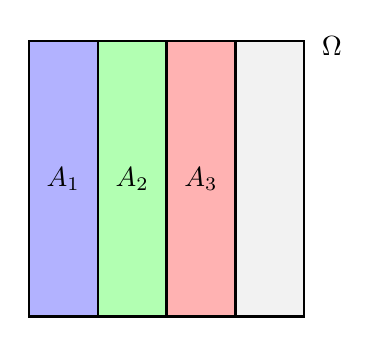
\begin{tikzpicture}[scale=3.5]
  		% Sample space
 		 \draw[thick] (0,0) rectangle (1,1);

		  % A1
		  \fill[blue!30] (0,0) rectangle (0.25,1);
		  \draw[thick] (0,0) rectangle (0.25,1);
		  \node at (0.125,0.5) {$A_1$};

		  % A2
		  \fill[green!30] (0.25,0) rectangle (0.5,1);
		  \draw[thick] (0.25,0) rectangle (0.5,1);
		  \node at (0.375,0.5) {$A_2$};

		  % A3
		  \fill[red!30] (0.5,0) rectangle (0.75,1);
		  \draw[thick] (0.5,0) rectangle (0.75,1);
		  \node at (0.625,0.5) {$A_3$};
	
		  % Remaining unassigned area
		  \fill[gray!10] (0.75,0) rectangle (1,1);
		  \draw[thick] (0.75,0) rectangle (1,1);
		  %\node at (0.875,0.5) {?};

		  % Omega label on top
		  \node at (1.1,0.98) {\textbf{$\Omega$}};
		\end{tikzpicture}
	\end{center}


Finite additivity gives:
\[\mathbb{P}(A_1\cup A_2\cup A_3)
= \frac14 + \frac14 + 0.3
= 0.8.\]

The remaining probability $0.2$ corresponds to the region $[0.8,1]\times[0,1]$ not assigned to any event.

\bigskip

%=======================================
%=======================================

%\textbf{Statement.}  
%For any event $A$,  
%\[
%\mathbb{P}(A^c)=1-\mathbb{P}(A).
%\]


\paragraph*{2. Complements Example:} (\textbf{Reliability of a Two-Component System})
\vskip 2mm  
Suppose a system works if at least one of its two independent components works.  
Let $A=\{\text{system fails}\}$.  
The system fails iff \emph{both} components fail:
\[
A = \{\text{component 1 fails}\}\cap\{\text{component 2 fails}\}.
\]
If each component has failure probability $p$, then
\[
\mathbb{P}(A)=p^2.
\]
Therefore the probability the system functions (the complement) is
\[
\mathbb{P}(A^c)=1-p^2.
\]
This complement rule is useful in reliability theory since failure events are often easier to characterize.

\begin{center}
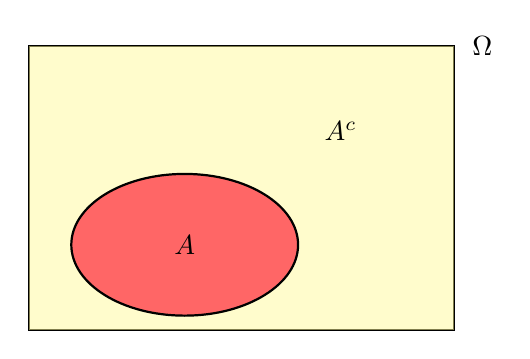
\begin{tikzpicture}[scale=1.8]
  % Universe
  \draw[thick] (0,0) rectangle (3,2);
  \node at (3.2,2) {$\Omega$};

  % A^c (complement) - yellow, semi-transparent
  \fill[yellow!40, opacity=0.5] (0,0) rectangle (3,2);
  \node at (2.2,1.4) {$A^c$};

  % A (system fails)
  \fill[red!60] (1.1,0.6) ellipse (0.8 and 0.5);
  \draw[thick] (1.1,0.6) ellipse (0.8 and 0.5);
  \node at (1.1,0.6) {$A$};
\end{tikzpicture}
\end{center}


\bigskip

%=======================================
%=======================================

%\textbf{Statement.}  
%For any event $A$,
%\[
%\mathbb{P}(A^c)=1-\mathbb{P}(A).
%\]

\paragraph*{3. Monotonicity Example:} (\textbf{Successes in Bernoulli trials})
\vskip 2mm  
Let $X$ be the number of successes in $n$ independent Bernoulli$(p)$ trials.  
Define events
\[
A=\{X\ge 3\}, \qquad B=\{X\ge 2\}.
\]
Since $A\subseteq B$, monotonicity gives
\[
\mathbb{P}(X\ge 3)\le \mathbb{P}(X\ge 2).
\]
This kind of containment underlies tail bounds and concentration inequalities.

\begin{center}
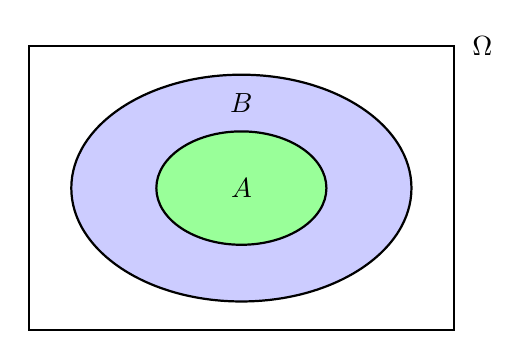
\begin{tikzpicture}[scale=1.8]
  % Universe
  \draw[thick] (0,0) rectangle (3,2);
  \node at (3.2,2) {$\Omega$};

  % B
  \fill[blue!20] (1.5,1) ellipse (1.2 and 0.8);
  \draw[thick] (1.5,1) ellipse (1.2 and 0.8);
  \node at (1.5,1.6) {$B$};

  % A subset inside B
  \fill[green!40] (1.5,1) ellipse (0.6 and 0.4);
  \draw[thick] (1.5,1) ellipse (0.6 and 0.4);
  \node at (1.5,1) {$A$};
\end{tikzpicture}
\end{center}

\bigskip


%=======================================
%=======================================

%\textbf{Statement.}  
%\[
%\mathbb{P}(A\cup B)
%= \mathbb{P}(A)+\mathbb{P}(B)-\mathbb{P}(A\cap B).
%\]

\paragraph*{4. Union of Two Events Example:} (\textbf{Password Characteristics})
\vskip 2mm
A website allows $N$ possible passwords.  
Let  
\[
A=\{\text{password contains a digit}\},\qquad
B=\{\text{password contains a special character}\}.
\]
If the password is generated uniformly at random, then
\[
\mathbb{P}(A\cup B)=\mathbb{P}(A)+\mathbb{P}(B)-\mathbb{P}(A\cap B),
\]
which correctly accounts for over-counting passwords that contain \emph{both} digits and special characters.  
This is the basis of many entropy and security calculations.
\begin{center}
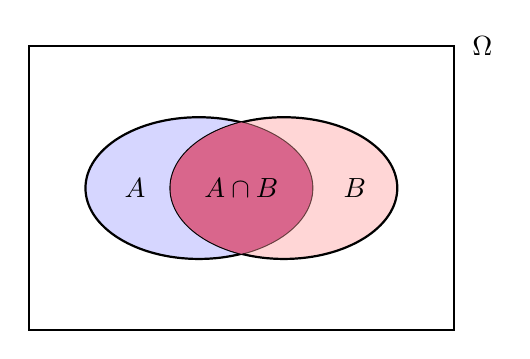
\begin{tikzpicture}[scale=1.8]

  % Universe
  \draw[thick] (0,0) rectangle (3,2);
  \node at (3.2,2) {$\Omega$};

  % --- Draw A and B first (with opacity) ---
  \fill[blue!40, opacity=0.4] (1.2,1) ellipse (0.8 and 0.5);
  \draw[thick] (1.2,1) ellipse (0.8 and 0.5);
  \node at (0.75,1) {$A$};

  \fill[red!40, opacity=0.4] (1.8,1) ellipse (0.8 and 0.5);
  \draw[thick] (1.8,1) ellipse (0.8 and 0.5);
  \node at (2.3,1) {$B$};

  % --- Now draw intersection shading (on top) ---
  \begin{scope}
    \clip (1.2,1) ellipse (0.8 and 0.5);
    \clip (1.8,1) ellipse (0.8 and 0.5);
    \fill[purple!60] (0,0) rectangle (3,2);
  \end{scope}

  % Label intersection
  \node at (1.5,1) {$A\cap B$};

\end{tikzpicture}
\end{center}


\bigskip


%=======================================
%=======================================

%\textbf{Statement.}  
%\[
%\mathbb{P}(A_1\cup A_2\cup A_3)
%= \sum_i \mathbb{P}(A_i)
%- \sum_{i<j}\mathbb{P}(A_i\cap A_j)
%+ \mathbb{P}(A_1\cap A_2\cap A_3).
%\]

\paragraph*{5. Inclusion--Exclusion Example (Three Sets):} (\textbf{3-Person Birthday Paradox})
\vskip 2mm  
Let $A_i=\{\text{person $i$ shares a birthday with someone else}\}$ in a group of 3, assuming 365 equally likely birthdays.  
One computes:
\[
\mathbb{P}(A_1)=\mathbb{P}(A_2)=\mathbb{P}(A_3)=\frac{364}{365},\quad\mathbb{P}(A_1\cap A_2)=\mathbb{P}(A_1\cap A_3)=\mathbb{P}(A_2\cap A_3)=\frac{1}{365},
\]
and
\[
\mathbb{P}(A_1\cap A_2\cap A_3)=\frac{1}{365^2}.
\]
Inclusion--exclusion gives the probability that at least two share a birthday:
\[
\mathbb{P}(A_1\cup A_2\cup A_3)
= 3\cdot\frac{364}{365}
- 3\cdot\frac{1}{365}
+ \frac{1}{365^2}.
\]
This avoids over-counting cases where multiple people share the same birthday.
\begin{center}
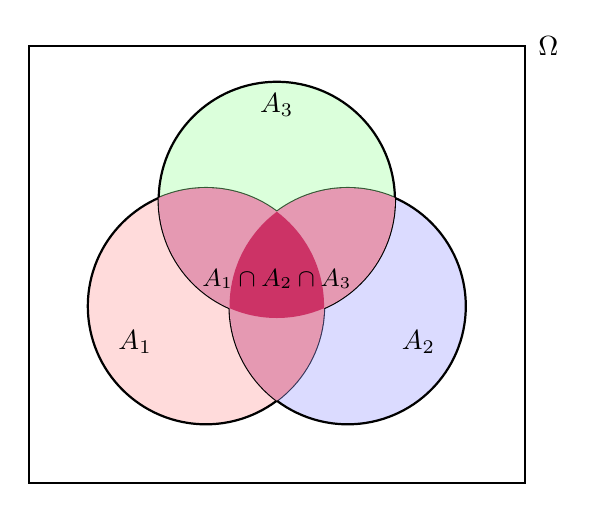
\begin{tikzpicture}[scale=1.5]

  % Universe
  \draw[thick] (-1.5,-1.5) rectangle (2.7,2.2);
  \node at (2.9,2.2) {$\Omega$};

  % --- 1. Draw sets with transparent fills ---
  \fill[red!40, opacity=0.35] (0,0) circle (1);
  \draw[thick] (0,0) circle (1);

  \fill[blue!40, opacity=0.35] (1.2,0) circle (1);
  \draw[thick] (1.2,0) circle (1);

  \fill[green!40, opacity=0.35] (0.6,0.9) circle (1);
  \draw[thick] (0.6,0.9) circle (1);

  % --- 2. Pairwise intersections ---
  \begin{scope}
    \clip (0,0) circle (1);
    \clip (1.2,0) circle (1);
    \fill[purple!40] (-1.5,-1.5) rectangle (2.7,2.2);
  \end{scope}

  \begin{scope}
    \clip (0,0) circle (1);
    \clip (0.6,0.9) circle (1);
    \fill[purple!40] (-1.5,-1.5) rectangle (2.7,2.2);
  \end{scope}

  \begin{scope}
    \clip (1.2,0) circle (1);
    \clip (0.6,0.9) circle (1);
    \fill[purple!40] (-1.5,-1.5) rectangle (2.7,2.2);
  \end{scope}

  % --- 3. Triple intersection ---
  \begin{scope}
    \clip (0,0) circle (1);
    \clip (1.2,0) circle (1);
    \clip (0.6,0.9) circle (1);
    \fill[purple!80] (-1.5,-1.5) rectangle (2.7,2.2);
  \end{scope}

  % Labels
  \node at (-0.6,-0.3) {$A_1$};
  \node at (1.8,-0.3) {$A_2$};
  \node at (0.6,1.7) {$A_3$};
  \node at (0.6,0.23) {\small $A_1\cap A_2\cap A_3$};

\end{tikzpicture}
\end{center}

\bigskip


%=======================================
%=======================================

%\textbf{Statement.}  
%If $B_1\supseteq B_2\supseteq B_3\supseteq\dots$, then
%\[
%\mathbb{P}\!\left(\bigcap_{n=1}^\infty B_n\right)
%= \lim_{n\to\infty} \mathbb{P}(B_n).
%\]

\paragraph*{6. Continuity of Probability Example:} (\textbf{Infinite Run of Heads})
\vskip 2mm   
Consider an infinite sequence of i.i.d.\ fair coin tosses.  
Let $B_n$ be the event
\[
B_n = \{\text{there is a run of $n$ consecutive heads at the start the sequence}\}.
\]
Then
\[
B_1 \supseteq B_2 \supseteq B_3 \supseteq \cdots.
\]

The event
\[
\bigcap_{n=1}^{\infty} B_n = \{\text{there exists a run of infinitely many consecutive heads}\}
\]
has probability
\[
\mathbb{P}\Big(\bigcap_{n=1}^{\infty} B_n\Big)=\ds\lim_{n\to\infty}\P(B_n)=\ds\lim_{n\to\infty}\ds\frac{1}{2^n}=0.
\]

\begin{center}
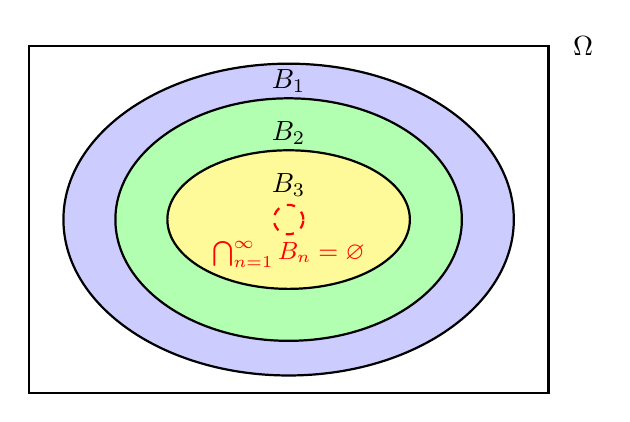
\begin{tikzpicture}[scale=2.2]

  % Universe
  \draw[thick] (0,0) rectangle (3,2);
  \node at (3.2,2) {$\Omega$};

  % B1: run of length 1
  \fill[blue!20] (1.5,1) ellipse (1.3 and 0.9);
  \draw[thick] (1.5,1) ellipse (1.3 and 0.9);
  \node at (1.5,1.8) {$B_1$};

  % B2: run of length 2
  \fill[green!30] (1.5,1) ellipse (1.0 and 0.7);
  \draw[thick] (1.5,1) ellipse (1.0 and 0.7);
  \node at (1.5,1.5) {$B_2$};

  % B3: run of length 3
  \fill[yellow!40] (1.5,1) ellipse (0.7 and 0.4);
  \draw[thick] (1.5,1) ellipse (0.7 and 0.4);
  \node at (1.5,1.2) {$B_3$};

  % Intersection of all B_n: impossible event
  \draw[red, thick, dashed] (1.5,1) circle (0.085);
  \node[red] at (1.5,0.8) {\small $\bigcap_{n=1}^{\infty} B_n = \varnothing$};

\end{tikzpicture}
\end{center}

However, for each finite $n$, a run of length $n$ eventually occurs almost surely:
\[
\mathbb{P}(B_n) = 1 \quad \text{for all finite } n.
\]

%%%%%%%%%%%%%%%%%%%%%%%%%%%%%%%%%%%%%%%%%%%%%%%%%%%%%%%%%%%%%%%%%%%%%%%%%%%%%%%%%%%%%%%%%
\section*{Practice Exercises:}
%%%%%%%%%%%%%%%%%%%%%%%%%%%%%%%%%%%%%%%%%%%%%%%%%%%%%%%%%%%%%%%%%%%%%%%%%%%%%%%%%%%%%%%%%

\textbf{Exercise 1 (Finite Additivity).}  
Let $\Omega = [0,1]^2$ and partition it into four horizontal strips:
\[
A_1 = [0,1]\times[0,1/4], \quad
A_2 = [0,1]\times[1/4,1/2], \quad
A_3 = [0,1]\times[1/2,3/4], \quad
A_4 = [0,1]\times[3/4,1].
\]
Compute $\mathbb{P}(A_1 \cup A_2 \cup A_3 \cup A_4)$ using finite additivity.

\bigskip

\textbf{Exercise 2 (Complements).}  
A fair six-sided die is rolled. Let $A$ be the event that an even number is rolled.  
\begin{enumerate}
    \item Compute $\mathbb{P}(A)$.
    \item Compute $\mathbb{P}(A^c)$ using the complement rule.
\end{enumerate}

\bigskip

\textbf{Exercise 3 (Monotonicity).}  
In a deck of 52 cards, let $A$ be the event ``drawing a face card" and $B$ be ``drawing a red card."  
\begin{enumerate}
    \item Are the events nested? Justify.
    \item Compare $\mathbb{P}(A)$ and $\mathbb{P}(B)$ using monotonicity if applicable.
\end{enumerate}

\bigskip

\textbf{Exercise 4 (Union of Two Events).}  
A bag contains 5 red balls and 3 blue balls. A ball is drawn at random.  
Let $A$ be the event ``red ball," and $B$ be the event ``numbered 3 or 4" (assume balls are numbered 1--8).  
\begin{enumerate}
    \item Compute $\mathbb{P}(A)$ and $\mathbb{P}(B)$.
    \item Compute $\mathbb{P}(A\cap B)$.
    \item Compute $\mathbb{P}(A\cup B)$ using the union formula.
\end{enumerate}

\bigskip

\textbf{Exercise 5 (Inclusion--Exclusion).}  
Three friends each independently pick a day of the week for a meeting. Let $A_i$ be the event that friend $i$ picks Monday.  
\begin{enumerate}
    \item Compute $\mathbb{P}(A_1)$, $\mathbb{P}(A_1 \cap A_2)$, and $\mathbb{P}(A_1 \cap A_2 \cap A_3)$.
    \item Using inclusion--exclusion, compute the probability that at least one friend picks Monday.
\end{enumerate}

\bigskip

\textbf{Exercise 6 (Continuity of Probability).}  
Consider an infinite sequence of independent tosses of a fair coin. Let $B_n$ be the event ``the first $n$ tosses are all heads."  
\begin{enumerate}
    \item Compute $\mathbb{P}(B_n)$ for $n=1,2,3$.
    \item Describe the relationship between the events $B_1, B_2, B_3, \dots$.
    \item Using continuity from above, explain what happens to $\mathbb{P}(B_n)$ as $n \to \infty$.
\end{enumerate}


\bigskip
\bigskip
\hrule
\bigskip

%%%%%%%%%%%%%%%%%%%%%%%%%%%%%%%%%%%%%%%%%%%%%%%%%%%%%%%%%%%%%%%%%%%%%%%%%%%%%%%%%%%%%%%%%
\section*{Solutions to Practice Exercises}
%%%%%%%%%%%%%%%%%%%%%%%%%%%%%%%%%%%%%%%%%%%%%%%%%%%%%%%%%%%%%%%%%%%%%%%%%%%%%%%%%%%%%%%%%


\textbf{Exercise 1 (Finite Additivity).}  

All four strips are disjoint and cover the whole square. Their probabilities are
\[
\mathbb{P}(A_1)=\mathbb{P}(A_2)=\mathbb{P}(A_3)=\mathbb{P}(A_4)=\frac{1}{4}.
\]
By finite additivity:
\[
\mathbb{P}(A_1 \cup A_2 \cup A_3 \cup A_4)
= \frac14 + \frac14 + \frac14 + \frac14 = 1.
\]

\bigskip

\textbf{Exercise 2 (Complements).}  

A fair six-sided die has outcomes $\{1,2,3,4,5,6\}$.  

\begin{enumerate}
    \item $A = \{2,4,6\} \implies \mathbb{P}(A) = \frac{3}{6} = \frac12$.
    \item $A^c = \{1,3,5\} \implies \mathbb{P}(A^c) = 1 - \mathbb{P}(A) = 1 - \frac12 = \frac12$.
\end{enumerate}

\bigskip

\textbf{Exercise 3 (Monotonicity).}  

\begin{enumerate}
    \item $A$ = face cards (12 cards), $B$ = red cards (26 cards). $A \not\subseteq B$ and $B \not\subseteq A$, so monotonicity does not directly apply.
    \item Nonetheless, $\mathbb{P}(A) = 12/52 = 3/13$, $\mathbb{P}(B) = 26/52 = 1/2$. One can see that $\mathbb{P}(A) < \mathbb{P}(B)$, consistent with intuitive containment (more red cards than face cards).
\end{enumerate}

\bigskip

\textbf{Exercise 4 (Union of Two Events).}  

\begin{enumerate}
    \item $A$ = red balls = 5 balls $\implies \mathbb{P}(A) = 5/8$.  
          $B$ = numbered 3 or 4 = 2 balls $\implies \mathbb{P}(B) = 2/8 = 1/4$.
    \item Intersection: red balls numbered 3 or 4 = assume numbers 1--5 are red, so red 3 and red 4 exist $\implies \mathbb{P}(A \cap B) = 2/8 = 1/4$.
    \item Union:
    \[
    \mathbb{P}(A \cup B) = \mathbb{P}(A) + \mathbb{P}(B) - \mathbb{P}(A \cap B)
    = \frac{5}{8} + \frac{2}{8} - \frac{2}{8} = \frac{5}{8}.
    \]
\end{enumerate}

\bigskip

\textbf{Exercise 5 (Inclusion--Exclusion).}  

\begin{enumerate}
    \item Each friend independently picks a day, 7 days in total:
    \[
    \mathbb{P}(A_1) = \frac{1}{7}, \quad 
    \mathbb{P}(A_1 \cap A_2) = \frac{1}{7^2}, \quad 
    \mathbb{P}(A_1 \cap A_2 \cap A_3) = \frac{1}{7^3}.
    \]
    \item By inclusion--exclusion:
    \begin{align*}
    \mathbb{P}(A_1 \cup A_2 \cup A_3)
    &= \sum_i \mathbb{P}(A_i) - \sum_{i<j} \mathbb{P}(A_i \cap A_j) + \mathbb{P}(A_1 \cap A_2 \cap A_3) \\
    &= 3 \cdot \frac{1}{7} - 3 \cdot \frac{1}{49} + \frac{1}{343} \\
    &= \frac{3}{7} - \frac{3}{49} + \frac{1}{343} \\
    &= \frac{147 - 21 + 1}{343} = \frac{127}{343}.
    \end{align*}
\end{enumerate}

\bigskip

\textbf{Exercise 6 (Continuity of Probability).}  

\begin{enumerate}
    \item $\mathbb{P}(B_1) = 1/2$, $\mathbb{P}(B_2) = (1/2)^2 = 1/4$, $\mathbb{P}(B_3) = (1/2)^3 = 1/8$.
    \item The events are decreasing: $B_1 \supset B_2 \supset B_3 \supset \dots$
    \item By continuity from above:
    \[
    \mathbb{P}\Big(\bigcap_{n=1}^\infty B_n\Big) = \lim_{n\to\infty} \mathbb{P}(B_n) = \lim_{n\to\infty} \left(\frac12\right)^n = 0.
    \]
    Hence, the probability of an infinite run of heads starting from the first toss is 0.
\end{enumerate}


%%%%%%%%%%%%%%%%%%%%%%%%%%%%%%%%%%%%%%%%%%%%%%%%%%%%%%%%%%%%%%%%%%%%%%%%%%%%%%%%%%%%%%%%%%%%%%%%%%%%%%
\section*{Selected (Optional) Proofs:}
%%%%%%%%%%%%%%%%%%%%%%%%%%%%%%%%%%%%%%%%%%%%%%%%%%%%%%%%%%%%%%%%%%%%%%%%%%%%%%%%%%%%%%%%%%%%%%%%%%%%%%

Let $(\Omega,\mathcal{F},\mathbb{P})$ be a probability space.  We present nontrivial examples for key consequences of the (Kolmogorov) probability axioms.

	\begin{itemize}
	
		\item {\bf\emph{Proof of Continuity:}} We prove the general continuity statement.
\vskip 1mm 
			\begin{proof}
Define the following:

\beq
B_1&=&A_1\\
B_2&=&A_2\setminus A_1\\
&\vdots&\\
B_n&=&A_n\setminus \left(\ds\bigcap^{n-1}_{i=1}A_i\right)
\eeq
It is clear that the $B_i$'s are disjoint; i.e., $B_k\cap B_j=\emptyset$ when $k\not=j$, and $\ds\cup^{\infty}_{i=1}A_i=\ds\cup^{\infty}_{i=1}B_i$ and $\ds\cup^{n}_{i=1}A_i=\ds\cup^{n}_{i=1}B_i$. But
\[\P\left(\ds\bigcup^{\infty}_{i=1}B_i\right)=\ds\sum^{\infty}_{i=1}\P(B_i)=\ds\lim_{n\to\infty}\ds\sum^{n}_{i=1}\P(B_i)=\ds\lim_{n\to\infty}\P\left(\ds\bigcup^{n}_{i=1}B_i\right)=\ds\lim_{n\to\infty}\P\left(\ds\bigcup^{n}_{i=1}A_i\right).\]
Then since $\ds\cup^{\infty}_{i=1}A_i=\ds\cup^{\infty}_{i=1}B_i$ we have completed the proof.\\
			\end{proof}
		
\ni We also have two special cases of continuity.

				\begin{enumerate}
			
					\item[(i)] If $A_1,A_2,\dots$ is an increasing sequence of events in $\F$; i.e., $A_i\subseteq A_{i+1}$ for all $i\in\N$, then		
\[\P\left(\ds\bigcup^{\infty}_{i=1}A_i\right)=\ds\lim_{n\to\infty}\P(A_n).\]

\ni It is easy to see that this is a special case of continuity since when $A_1,A_2,A_3,\dots$ is an increasing sequence, then $\ds\cup^{n}_{i=1}A_i=A_n$.\\ 
				
					\item[(ii)] If $A_1,A_2,\dots$ is a decreasing sequence of events in $\F$; i.e., $A_{i+1}\subseteq A_i$ for all $i\in\N$, then		
\[\P\left(\ds\bigcap^{\infty}_{i=1}A_i\right)=\ds\lim_{n\to\infty}\P(A_n).\]
				
\ni This follows from property(i) and DeMorgan's Rule.
				
				\end{enumerate}
			
		\item {\bf\emph{Proof of Union Bound:}} We prove the union bound result, but first observe it is only useful when $\ds\sum^{\infty}_{i=1}\P(A_i)<1$.
\vskip 1mm
\begin{proof}
Let $B_n=A_n\setminus \left(\ds\bigcap^{n-1}_{i=1}A_i\right)$ for all $n\in\N$, so that $\ds\cup^{\infty}_{i=1}A_i=\ds\cup^{\infty}_{i=1}B_i$. Then we have
\[\P\left(\ds\bigcup^{\infty}_{i=1}A_i\right)=\P\left(\ds\bigcup^{\infty}_{i=1}B_i\right)=\ds\lim_{n\to\infty}\ds\sum^{n}_{i=1}\P(B_i)\le\ds\lim_{n\to\infty}\ds\sum^{n}_{i=1}\P(A_i)=\ds\sum^{\infty}_{i=1}\P(A_i),\]
where the inequality follows because $B_i\subseteq A_i$ for each $i\ge 1$. This completes the proof.\\
\end{proof}

		\item  {\bf\emph{Proof of Borel-Cantelli Lemma \#1:}} 
\vskip 1mm  			
We will prove this first lemma, but first consider an example. Consider the experiment of an infinite series of coin flips, so that $\O=\{0,1\}^{\infty}$, and let $A_n$ be the event that the $n$th toss is heads. Then if $\P$ is a probability measure on $(\O,\F)$ such that $\P(A_n)=1/n^2$ for all $n\ge 1$, we have $\sum^{\infty}_{n=1}A_n<\infty$. Then almost surely only finitely many heads will occur in the infinite string of coin tosses.

				\begin{proof}
Observe that the event $A$ that infinitely many $A_i$'s occur can be written as
\[A=\ds\bigcap^{\infty}_{n=1}\ds\bigcup^{\infty}_{i=n}A_i.\]
Then let $B_n=\bigcup^{\infty}_{i=n}A_i$ so that $A=\bigcap^{\infty}_{n=1}B_n$. To clarify, this event is the event that, for any $n$, at least one of the $A_m$ (where $m\ge n$) will occur. Clearly, $B_i\subset B_{i+1}$, and so the sequence $B_1,B_2,\dots$ is an increasing sequence. Therefore, assuming that $\sum^{\infty}_{i=1}\P(A_i)<\infty$, we have
\beq
\P\left(\ds\bigcap^{\infty}_{n=1}B_n\right)&=&\ds\lim_{n\to\infty}\P(B_n)\qquad\text{(by continuity)}\\
&=&\ds\lim_{n\to\infty}\P(\left(\ds\bigcup^{\infty}_{i=n}A_i\right)\\
&\le&\ds\lim_{n\to\infty}\ds\sum^{\infty}_{i=n}\P(A_i)\quad\text{(by union bound)}\\
&=&0
\eeq
The last inequality follows because the series converges to a finite value. This completes the proof.\\
				\end{proof}
				
		\item  {\bf\emph{Proof of Borel-Cantelli \#2:}} We won't prove this result.
			\begin{lemma}[BC Lemma \#2] If $A_1,A_2,\dots$ is a sequence of independent events in $\F$ such that $\sum^{\infty}_{i=1}\P(A_i)=\infty$, then almost surely (or with probability one) infinitely many of the $A_i$ will occur.			
			\end{lemma}
			
%			\begin{ex} Consider the experiment of an infinite series of coin flips, so that $\O=\{0,1\}^{\infty}$, and let $A_n$ be the event that the $n$th toss is heads. Then if $\P$ is a probability measure on $(\O,\F)$ such that $\P(A_n)=p>0$ for all $n\ge 1$, we have $\sum^{\infty}_{n=1}A_n=\infty$. Then almost surely infinitely many heads will occur in the infinite string of coin tosses.
%			\end{ex}
 				
	\end{itemize}
	

%%%%%%%%%%%%%%%%%%%%%%%%%%%%%%%%%%%%%%%%%%%%%%%%%%%%%%%%%%%%%%%%%%%%%%%%%%%%%%%%%%%%%%%%%%%%%%%%%%%%%%%
%\section*{The R Code:} 
%%%%%%%%%%%%%%%%%%%%%%%%%%%%%%%%%%%%%%%%%%%%%%%%%%%%%%%%%%%%%%%%%%%%%%%%%%%%%%%%%%%%%%%%%%%%%%%%%%%%%%%
% Here is the R code used for the above simulations.
%\vspace*{2mm}
%\small 
%\begin{lstlisting}[language=R]
%
%
%
%\end{lstlisting}



\vskip 1cm
\hrule
\vskip 5mm
\begin{center}
\bf Please let me know if you have any questions, comments, or corrections!
\end{center}

%%%%%%%%%%%%%%%%%%%%%%%%%%%%%%%%%%%%%%%%%%%%%%%%%%%%%%
\end{document}
%%%%%%%%%%%%%%%%%%%%%%%%%%%%%%%%%%%%%%%%%%%%%%%%%%%%%%
